\documentclass[AutoFakeBold=2.5]{myclass}
\usepackage{lipsum} 
\begin{document}

% 1. 生成封面
% 确保文件夹里放了一张名为 logo.png (或 logo.jpg) 的图片,否则会报错
\makecover 

\Englishmakecover
% 2. 正文部分测试
\setcounter{page}{1} % 重置页码
\pagenumbering{Roman} % 使用罗马数字页码

\begin{cnabstract}

摘要是论文(设计)内容不加注释和评论的简短陈述,应具有独立性和自明
性,即不阅读论文(设计)的全文,就可以获得必要的信息。

摘要一般应说明研究工作的目的 和意义、研究思想和方法、研究过程、研究
结果和最终结论等。摘要中一般不用图、表、化学结构式、计算机程序,不用非
公知公用的符号、术语和非法定的计量单位。

中文摘要一般为 300~500 汉字。

摘要页置于英文题名页后。

关键词是从论文(设计)题名、摘要或正文中选取的对表示论文(设计)主
题内容起关键作用,且具有检索意义的词或词组。一般每篇论文(设计)应选取
3~5 个词作为关键词,以显著的字符另起一行,排在同种语言摘要的下方,尽量用
《汉语主题词表》或各专业主题词表提供的规范词。

关键词与摘要的内容之间空一行。关键词的词间用分号间隔,末尾不加标点。

\end{cnabstract}

\cnkeywords{关键词一;关键词二;关键词三}

% 英文摘要
\begin{enabstract}
This is the English abstract. The abstract should be a concise summary of the thesis (design), providing an overview of the research purpose, methodology, process, results, and conclusions. It should be self-contained and independent, allowing readers to grasp the essential information without reading the full text.

Figures, tables, chemical structural formulas, computer programs, non-public symbols, terms, and non-statutory measurement units should generally not be used in the abstract.

The English abstract is typically 300-500 words and is placed after the English title page.
\end{enabstract}
\enkeywords{Keyword One; Keyword Two; Keyword Three}


\tableofcontents

% 5. 正文部分(需要手动添加目录条目)

\setcounter{page}{1} % 重置页码
\pagenumbering{arabic} % 使用阿拉伯数字页码
\pagestyle{fancy}

% 设置行距为20pt
\zihao{-4}
\setlength{\baselineskip}{20pt}
\selectfont
\section{荷载算}
\subsection{基本载荷取值}

\subsubsection{活载取值}
根据《荷载规范》,本工程上人屋面活荷载取为 \(q_w = 1.5 KN/m^2\)。

晨曦初露,薄雾如纱般轻轻覆在沉睡的小城之上。青石板路还留着昨夜的雨痕,深深浅浅的水洼里,倒映着灰白的天和翘起的飞檐。早起的老人推着吱呀作响的自行车走过,车篮里一把嫩绿的青菜还滴着水珠。巷口那家早点铺的蒸汽最先升起来,混着油条的焦香和豆浆的醇厚,一丝丝、一缕缕地渗进潮湿的空气里。

\subsubsection{测试测试}

\subsection{研究意义}
研究意义的内容...

\section{文献综述}
\subsection{国内外研究现状}
文献综述内容...

\subsection{研究评述}
研究评述内容...

\section{研究方法}
\subsection{研究方法设计}
风载体型系数$\mu_s$:.....;风振系数:xxxxxxxxxxxxxxxx有:很久很久以前有一只小马,小马要过河,但是他不知道水的深浅,于是他问过路的牛,牛说:“我经常过河,水很浅,你放心大胆地走吧!”小马听了牛的话,就放心大胆地走进了河里,结果淹死了。后来小马的朋友小羊也要过河,他也问了牛,牛还是那样说的。小羊听了牛的话,也放心大胆地走进了河里,结果也淹死了。后来小马和小羊的朋友小猪也要过河,他也问了牛,牛还是那样说的。小猪听了牛的话,也放心大胆地走进了河里,结果也淹死了。后来小马、小羊和小猪的朋友小狗也要过河,他也问了牛,牛还是那样说的。小狗听了牛的话,也放心大胆地走进了河里,结果也淹死了。后来小马、小羊、小猪和小狗的朋友小猫也要过河,他也问了牛,牛还是那样说的。小猫听了牛的话,也放心大胆地走进了河里,结果也淹死了。后来小马、小羊、小猪、小狗和小猫的朋友小鸡也要过河,他也问了牛,牛还是那样说的。小鸡听了牛的话,也放心大胆地走进了河里,结果也淹死了。于是小马问妈妈:“妈妈,为什么我们都淹死了?”妈妈说:“因为牛是瞎的,它根本不知道水有多深,它只是想骗你们过河,好吃掉你们而已!”从此以后,小动物们再也不相信牛的话了。
\begin{equation}
W=\mu_{s} \cdot \mu_{z} \cdot \beta_{z}=...
\end{equation}

所以说我们要谨慎行事,不能盲目相信他人的话。
\begin{table}[htbp]
    \centering
    \caption{左风作用下荷载计算}
    \label{tab:wind_load}

    % 定义 Y 列格式:居中 (centering) + 自动宽度 (X)
    \newcolumntype{Y}{>{\centering\arraybackslash}X} 

    % 使用 tabularx 环境,总宽度设为 \textwidth
    \begin{tabularx}{\textwidth}{YYYYYYYY} 
        \toprule 
        层次 & $Z(m)$ & $\mu_z$ & $\beta_z$ & $\mu_s$ & $\omega_0 (kN/m^2)$ & $A(m^2)$ & $P_{\omega}(kN)$ \\
        \midrule
        1 & 4.5  & 1.00 & 1.42 & 0.8 & 0.45 & 24.0 & 12.27 \\
        2 & 7.8  & 1.15 & 1.56 & 0.8 & 0.45 & 24.0 & 15.50 \\
        3 & 11.1 & 1.32 & 1.68 & 0.8 & 0.45 & 24.0 & 19.16 \\
        \midrule
        合计 & - & - & - & - & - & 72.0 & 46.93 \\
        \bottomrule
    \end{tabularx}
\end{table}

从前有一只狐狸,它非常狡猾。有一天,它被一只老虎抓住了。狐狸对老虎说:“你不能吃我,因为我是天帝派来管理百兽的使者。如果你吃了我,天帝会惩罚你的。”老虎半信半疑,于是狐狸让老虎跟着它一起去森林\citet{rr}里巡视。路上,狐狸看到其他动物都害怕地逃跑了,老虎以为是因为狐狸的身份,便更加相信了狐狸的话。最后,老虎放了狐狸,自己也成了森林里的霸主。从此以后,狐狸利用老虎的威风,吓唬其他动物,过上了逍遥自在的生活。

有一天,一个农夫在路上发现了一条冻僵的蛇。出于同情,农夫把蛇捡起来,放在怀里取暖。蛇渐渐苏醒过来,感激地对农夫说:“谢谢你救了我。”然而,当农夫放下蛇时,蛇突然咬了他一口。农夫痛苦地问:“为什么你要咬我?我救了你啊!”蛇冷冷地回答:“这是我的本性,你不该相信我。”农夫最终因为伤口感染而去世。这个故事告诉我们,有些本性难改,我们应该谨慎对待那些天性凶恶的人或事物。
\begin{figure}[htb]
    \centering
    % 插入图片:width=0.8\textwidth 表示宽度占页面的 80%
    % {figure/dd.svg} 是图片路径,请确保你文件夹里有这个图
    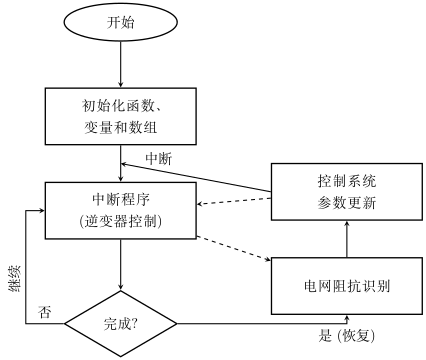
\includegraphics[width=0.8\textwidth]{figure/dd.pdf}
    
    % 标题 (会自动变成:图 1.1 这是一个示例图片)
    \caption{这是一个示例图片}
\end{figure}

哈哈哈哈哈哈哈哈哈
\subsection{实验方案}
实验方案内容...

\section{研究结果与分析}
\subsection{实验结果}
结果内容...

\subsection{结果分析}
分析内容...

\section{结论与展望}
\subsection{研究结论}
结论内容...

\subsection{研究展望}
展望内容...
\bibliographystyle{gbt7714-numerical}
\bibliography{ref}

\end{document}